\section{Detailed Design Optical Emitting Payload} 
\label{sec:DDlaser}
\acs{LiDAR} is a remote sensing system comprising an optical emitting device, used to acquire topographic data, e.g. surface elevation gradients or ground composition by evaluating the \acs{BRDF}, considering multi-angular measurement are taken. For the generation of optical pulses, a highly efficient, diode-pumped, solid-state Nd-YAG \acs{laser} is considered \ac{DPSSL}. Solid-State \acp{laser} have a high \acs{TRL} with relatively good properties in terms of beam quality (Q-factor), efficiency and pulse manipulation. Data products for topographical missions require that the \ac{laser} wave form be nearly pure Gaussian (known as transverse mode $TEM_(00)$), both temporally and spatially, with a uniform wave front. The digitized time of flight waveform returning provides the topographic structure \cite{nd_yag_life}.

\subsection{Principles of \textit{AlGaAs} Laser Diodes}
\label{laser_diodes}
\acs{laser} diodes are electrically pumped semiconductor \acp{laser}, in which the gain is generated by an electrical current flowing through a \textit{p-n junction} or (more frequently) a \textit{p-i-n structure}\cite{lasertech}. In such a heterostructure, excitons dynamics can occur (electrons and holes can recombine), releasing the energy portions as photons. This process can be spontaneous, but can also be stimulated by incident photons, in effect leading to optical amplification. Most higher-power \acs{laser} diodes, however, exhibit a relatively poor beam quality, combined with other non-favorable properties, such as a large beam divergence, high asymmetry of beam radius and beam quality between two perpendicular directions, and astigmatism (property of rays to exhibit different foci in different symmetrical planes). Especially considering the long distances used in \acs{LiDAR} missions, these properties degrade the potential data quantity, as well as quality.

\begin{figure} [ht]
\centering
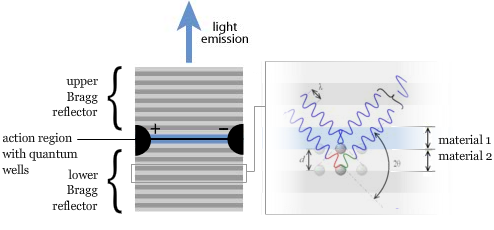
\includegraphics[scale=0.5]{chapters/img/diodelaser.png}	
\caption{Basic diode laser configuration \cite{laser_power} }
\label{laser_power}
\end{figure}

A quantum well is a thin layer which can confine (quasi-)particles (typically electrons or holes) in the dimension perpendicular to the layer surface, whereas the movement in the other dimensions is not restricted. A quantum well is often realized with a thin layer of a semiconductor medium, embedded between other semiconductor layers of wider bandgap. The thickness of such a quantum well is typically $\sim$5 - 20 [nm]. 

A major challenge is to reach the laser threshold, because the optical gain for the intracavity laser beam occurs only on a very small distance (in one or several quantum wells). It is therefore necessary to realize a laser resonator with very low losses, i.e., \textit{Bragg mirrors} with high reflectivity. A Bragg mirror (also called \textit{distributed Bragg reflector} is a structure which consists of an alternating sequence of layers of two different optical materials. The principle of operation can be understood as follows. Each interface between the two materials contributes a Fresnel reflection. For the design wavelength, the optical path length difference between reflections from subsequent interfaces is half the wavelength; in addition, the reflection coefficients for the interfaces have alternating signs. Therefore, all reflected components from the interfaces interfere constructively, which results in a strong reflection. The reflectivity achieved is determined by the number of layer pairs and by the refractive index contrast between the layer materials. 

Individual \acs{laser} diodes normally generate continuous waves with powers $\sim$ 1 - 10 [mW]. To be able to generate higher power ($\sim$1 - 10 [W]) \textit{laser diodes arrays} or \textit{laser diode stacks} can be created, simply be combining multiple individual \acs{laser} diodes. High-power laser diode arrays \ac(LDAs) are used for a variety of space-based remote sensor laser programs as an energy source for \acp{DPSSL}. \acp{LDA} have been flown on NASA missions including MOLA, GLAS and MLA and have continued to be viewed as an important part of the \acs{laser}-based instrument component suite \cite{lda_main}. 

Laser diode bars have many single emitters arranged side-by-side and spaced approximately 0.5 [mm] apart, on a single slab of semiconductor material measuring approximately 0.5 [mm] x 10 [mm] in size. The individual emitters are connected in parallel which keeps the required voltage low at ~2V, but increases the required current to ~50 A/bar to 100 A/bar. Stacking these laser diode bars 2 to 20+ slabs high yields high power \acp{LDA} capable of emitting several hundreds of Watts. Electrically, the bars are wired in series increasing the voltage by 2 V/bar while maintaining the total current at ~50 A to 100 A. These arrays are one of the enabling technologies for efficient, high power solid-state lasers.

Traditionally these arrays are operated in QCW (Quasi Continuous Wave) mode with pulse widths of ~50 �s to 200 �s and repetition rates of ~10 Hz to 200 Hz. In QCW mode, the wavelength and the output power of the laser reaches steady-state but the temperature does not. The advantage is a substantially higher output power than in CW mode, where the output power would be limited by the internal heating and the heat sinking properties of the device. The disadvantage is a much higher thermally induced mechanical stress caused by the constant heating and cooling cycle of the QCW operational mode.

Considering the fact that Nd:YAG is considered as gain medium (\ref{nd_yag}), the existence of strong $Nd^{3+}$ absorption near 808 [nm] permits efficient pumping with a GaAlAs (Gallium-Aluminium-Arsenide) diode \acp{laser} for the $F_{3/2}\rightarrow I_{9/2}$ transition. The direct band gap crystal AlGaAs is often used for laser diodes with wavelengths between
750nm and 880nm. $Al_{x}Ga_(1-x)As$, through changing the x, the ratio of the aluminium
to gallium can be adjusted to vary the band gap and thereby control the wavelength. In the double heterostructure, stimulated emission occurs only within a thin active
layer of GaAs, which is sandwiched between p- and n- doped AlGaAs layers that have
a wider band gap. Laser diodes use heterojunctions to achieve simultaneous carrier and
photon confinement in the active region. 

\begin{figure} [ht]
\centering
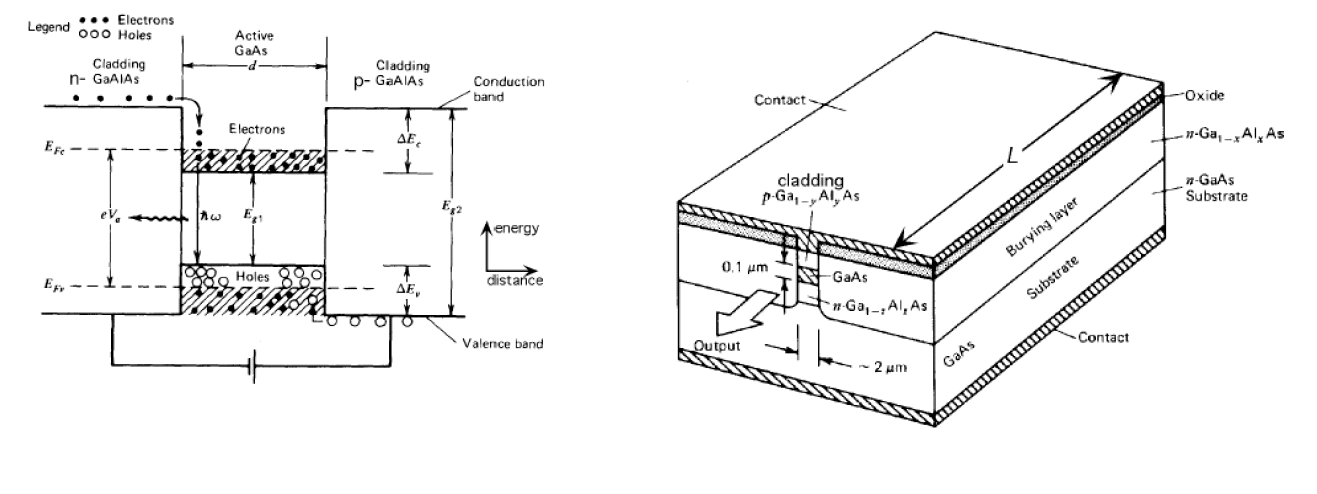
\includegraphics[scale=0.5]{chapters/img/laser_diode_algaas.png}	
\caption{\cite{algaasdiodes}}
\label{laser_power}
\end{figure}

A high laser efficiency demands that the light and injected charge carriers be confined as closely as possible to the same volume. The AlGaAs daser diode consists of a double heterojunction formed by an undoped (or lightly p-doped) active region surrounded by high bandgap p and n $Al_{x}Ga_(1-x)As$ cladding layers \cite{algaasdiodes}. The surrounding cladding layers provide an energy barrier to confine carriers to the active region. The actual operation wavelengths may range from 750 � 880 [nm] due to the effects of dopants, the size of the active region, and the compositions of the active and cladding layers. When a certain parameter is fixed, the wavelength can vary in several nanometers due to other variables. For example, when the active layer has an energy gap $E_{g} = 1.424 [eV]$, the nominal emission wavelength is $\lambda = hc/E_{g}= 871 [nm]$. When a bias voltage is applied in the forward direction, electrons and holes are injected into the active layer. Since the band gap energy is larger in the cladding layers than in the active layer, the injected electrons and holes are prevented from diffusing across the junction by the potential barriers formed between the active layer and cladding layers. The electrons and holes confined to the active layer create a state of population inversion, allowing the amplification of light by stimulated emission.

\begin{figure} [ht]
\centering
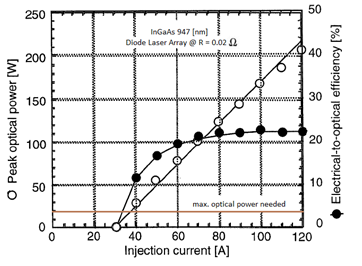
\includegraphics[scale=1.0]{chapters/img/laser_power.png}	
\caption{laser power \cite{diodepower} }
\label{laser_power}
\end{figure}

\subsection{Diode Pumped Solid-State Laser Configuration} 
\label{laserconfig}

\begin{figure} [ht]
\centering
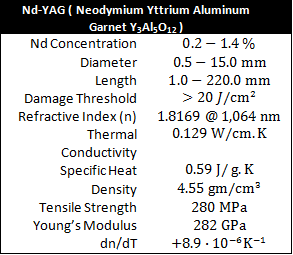
\includegraphics[scale=1.2]{chapters/img/laser_configuration.png}	
\caption{laser configuration}
\label{laser}
\end{figure}

\subsubsection{Nd-YAG Laser Characteristics}
\label{nd_yag}
\textit{Yttrium Aluminum Garnet} has emerged as the most widely produced laser gain host and has enjoyed recent popularity as a substrate material for optical components. The YAG host is a stable compound, mechanically robust, physically hard, optically isotropic, and transparent from below 300 to beyond 4,000 [nm]. YAG single crystals are able to accept trivalent laser activator ions from both the rare Earth and transition metal groups, and can be grown with very low strain.

For applications where $TEM_{00}$ single mode operation is required, it is necessary to reduce or eliminate the variations in the bulk material and in the absorption of the pumping radiation throughout the component. In addition, wavefront distortions due to geometric imperfections and thermal gradient effects such as thermal lensing must be minimized. In this case, Neodymium concentration in the 0.4 to 0.8\% range is typically specified.

\begin{figure} [ht]
\centering
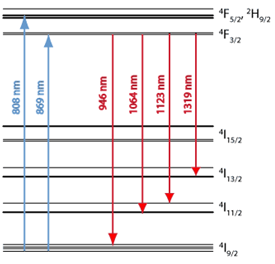
\includegraphics[scale=1.2]{chapters/img/laser_line.png}	
\caption{laser line}
\label{laser}
\end{figure}

\subsubsection{Second Harmonic Generation}
\label{SHG}
Since Nd-YAG has no principle absorption peak at the desired wavelength for the \acs{LiDAR} mission, the frequency should be altered from the original 946 [nm]. This can be done using \textit{second harmonic generation} or \textit{frequency doubling} in nonlinear crystals.
The physical mechanism behind frequency doubling can be understood as follows. Due to the ��(2) nonlinearity, the fundamental (pump) wave generates a nonlinear polarization wave which oscillates with twice the fundamental frequency. According to Maxwell's equations, this nonlinear polarization wave radiates an electromagnetic field with this doubled frequency. Due to phase-matching issues, the generated second-harmonic field propagates dominantly in the direction of the nonlinear polarization wave. The latter also interacts with the fundamental wave, so that the pump wave can be attenuated (pump depletion) when the second-harmonic intensity develops: energy is transferred from the pump wave to the second-harmonic wave.

\subsubsection{Pulse Generation}
\label{pockel}
The generation and manipulation of pulses can highly influent the data in \acs{LiDAR} missions. To be able to transform the continuous wave into a pulsed wave, Q-switching is applied. Q-switching is a technique for obtaining energetic short pulses from a laser by modulating the intracavity losses and thus the Q-factor (a measure of the damping of resonator modes) of the laser resonator. The technique is mainly applied for the generation of nanosecond pulses of high energy and peak power with solid-state bulk lasers. For \textit{active Q-switching}, the losses are modulated with an active control element typically either an acousto-optic or electro-optic modulator. Both techniques rely on the fact that the optical properties within a nonlinear crystal change on the occurrence of an induced sound wave (acousto-optic) or electric field (electro-optic). There are also mechanical Q-switches such as spinning mirrors, used as end mirrors of laser resonators. In any case, the achieved pulse energy and pulse duration depends on the energy stored in the gain medium, i.e. on the pump power and the pulse repetition rate.  A Pockels cell is a device consisting of an electro-optic crystal (with some electrodes attached to it) through which a light beam can propagate. Dependent on the configuration, the phase delay or polarization state in the crystal (due to the \textit{Pockels effect}) can be modulated by applying a variable electric voltage.  Hence, for short periods (dt) the polarization state of the incoming electromagnetic radiation can be altered. If a \textit{polarizer disk} is used after the Pockel cell, the generation of pulses will begin, since the polarizer disk transmits certain polarized states only, deflecting the rest (acting like a 'polarize filter'). Pulses in the order of nanoseconds could be created this way. Care should be taken at the fact that the peak power after the Pockel cell is increased in several orders, due to the conversion from continuous to pulsed waves. Hence, the polarizer disk should be able to cope with these stresses.

\begin{figure} [ht]
\centering
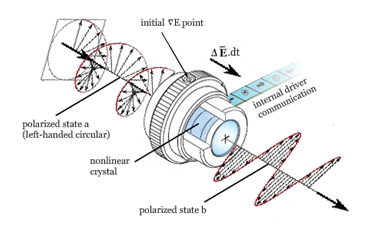
\includegraphics[scale=1.2]{chapters/img/laser_polarized.png}	
\caption{laser polarized}
\label{laser}
\end{figure}

\subsection{Optical Characteristics} 
\label{opticalchar}
The radius of the beam equals 400 [$\mu$m]. Considering a $TEM_{00}$ transverse mode of electromagnetic radiation this results in a area equal to 
\begin{equation}
\label{area}
A_{beam} = \pi \cdot r^{2} = \pi \cdot 400^{2} = 502,654 \mu m^{2} = 0.50265 cm^{2}
\end{equation}

The pulse energy $E_{p}$ [J] (maximum optical power of a pulse) is determined using the simulator. Sufficient energy should be present within the electromagnetic radiation to ensure the optimum path from the transmitter towards the receiver. Lowering the value of $E_{p}$ below this threshold energy can lead to atmospheric and surface absorption or translational mismatching due to incorrect scattering. The value of $E_{p}$ of this particular mission is determined to be $\sim$1 [mJ] (see \ref{simulator}).
Pulse repetition rate $f_{rep}$ [Hz], i.e. the number of pulses emitted per second, is an important parameter for the altimetry mission. Again, using the results from the simulator, the quantity of this parameter can be determined to be $\sim$5000 [Hz] ($\Delta$t = 0.0002 [s] with a pulse duration $t_{p}$ $\sim$10 [ns]). Using the value of $f_{rep}$, the spatial resolution of the pulses along-track and in the nadir-direction can be calculated, considering the orbital velocity to be fixed at the determined altitude.  
\begin{equation}
\label{alongtrackres}
d_{along} = \Delta t \cdot v = 0.0002 [s] \cdot 7,617 [m/s] = 1.5234 [m]
\end{equation}

\begin{equation}
\label{alongtracknadir}
d_{nadir} = \Delta t \cdot c = 0.0002 [s] \cdot 299,792,458 [m/s] = 59,958.49 [m]
\end{equation}

Considering the value of $E_{p}$ to be 1 [mJ] with a $f_{rep}$ of 5,000 [Hz], the total power that should be induced within the electromagnetic wave can be calculated.
\begin{equation}
\label{outputpower}
P_{output} = E_{p} \cdot f_{rep} = 0.001 [J] \cdot 5,000[1/s] = 5.0 [W]
\end{equation}

Input power equals output power times efficiency = $16 W \times eff = ((0.35)*(0.99)^6)$
The pulse peak intensity equals $E_{p}/t_{p} = 0.001 [J] / 10\cdot10^{-9} [s] = 100,000 W$. The intensity turns out to be $\frac{E_{p}/t_{p}}{A_{beam}} = \frac{100,000 [W]}{0.50265 [cm^{2}]} = 198,950.6 [W/cm^{2}] (0.00199 [J/cm^{2}/10ns])$. The standard damage threshold energy $E_{p,damage}$for dielectric components equals $0.5 - 10 [J/cm^{2}/10 ns]$. Considering the lowest value $I_{p,damage}$, hence, $0.5 [J/cm^{2}/10 ns]$, and converting this to the appropriate dimensions, shows the intensity created within the electromagnetic pulses should do no harm to the dielectric components. Especially the polarizer disk (with the lowest $I_{p,damage}$) is vulnerable for peak power caused by pulsed electromagnetic radiation. 

\subsection{Gaussian Beam Propagation and Diffraction}
\label{diff}
In most \acs{laser} applications, the intensity spatial distribution of the beam can be approximated by assuming that the \acs{laser} beam has an Gaussian intensity profile, which corresponds to the theoretical $TEM_{00}$ transverse mode. Unfortunately, the output from real-life \acp{laser} in not truly Gaussian. To accommodate this invariance, a quality factor, $M^{2}$ has been defined to describe the deviation of the \acs{laser} beam from a theoretical Gaussian. For high-energy multimode \acp{laser} the $M^{2}$ factor can be high as 25 - 30. The fun

Diffraction occurs when a wavefront(radiant beam)impinges upon the edge of an opaque screen or aperture. Light appears outside the perfect geometrical shadow because the light has been diffracted by the edge of the aperture. The effect this has on our simple rotationally symmetric optical systems is that a point does not map to a point, but is blurred or smeared.\cite{prism_book} 

\begin{figure}[ht!]
\centering
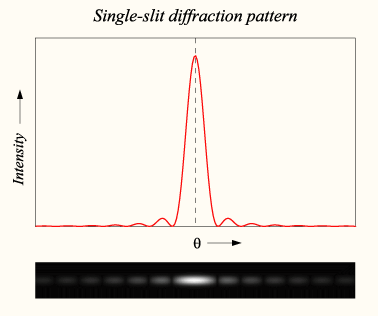
\includegraphics[scale = 0.8]{chapters/img/diffraction_singleslit.png}
\caption{Single-slit diffraction pattern.}
\label{fig:single_slit}
\end{figure}

In far-field case, where the pattern observed is a long distance from the aperture, it is known as Fraunhofer diffraction. The patterns caused by diffraction can be analyzed via Fourier optics of a circular aperture for rotationally symmetric optical systems. The results are in the form of a Bessel function, which is shown as figure \ref{fig:single_slit} on page \ref{fig:single_slit} for single-slit diffraction. Therefore, the actual radiant energy distribution in the image of a point differs from the point because of diffraction. This diffraction spot is called the "Airy disc", a three-dimensional representation of which is given in figure \ref{fig:airydisk} on page \ref{fig:airydisk} by definition or accepted practice. About 84\% of the radiant power is contained in this central disc. The diffraction limit is the ultimate design criterion as to how well the optical system creates an image. The diffraction limit is described as angular resolution, $\theta$, for half of the diffraction blur, which can be expressed as equation \ref{diffraction}. where D is the diameter of the aperture and $\lambda$ is the light wavelength.

\begin{equation}
\label{diffraction}
\theta = 1.22\frac{\lambda}{D}
\end {equation}

\begin{figure}[ht!]
\centering

\includegraphics[scale = 0.15]{chapters/img/diffraction_airydisk.png}
\caption{Airy disk pattern.}
\label{fig:airydisk}
\end{figure}

To compare with previous earth observation mission \acs{ICEsat}, which produces 70 meters diameter laser spot, 10[mm] laser diameter can produce about 60 meters diameter without focusing system. 

\subsection{Thermal Control} 
\label{opticalthermal}
Basically, there are three critical parts (\acs{LDA}, Nd:YAG \acs{laser} crystal and optical components after polarizer disk) of the \acs{laser} configuration in terms of thermal control. All of these components shall be considered in this subsection.

\textit{\acs{LDA}}.
The constituent parts and materials of a typical \acs{LDA} are the diode die (laser bar) and the packaging materials. The packaging design and materials enable the array of laser bars to stay together in a stack, to be energized electrically (with a relatively high drive current), to pass the heat generated out of the unit to the mounting surface (thermal path, heat sinking), to be sufficiently rugged against mechanical insults, to provide a standard mounting interface (screws or clamps) and to be as small as possible. The active region of the LDA, where heat is generated, is only about 1 micron wide, located about 3 microns from the P side of the bar. The bars are about 0.1 mm wide and typically spaced about 0.5 mm from each other. Waste energy in the form of heat must be conductively transferred into the solder material and from there into the heat sink material (typically BeO or CuW) as rapidly as possible. The solder material of choice is a soft Indium alloy for its ductile property allowing the bar and the heat sink to expand or contract at different rate with temperature. The \acs{LDA} manufacturers try to use materials which possess higher thermal conductivity and a relatively comparable coefficient of thermal expansion (CTE) in order to minimize the thermal resistance of the device and the induced mechanical stresses. Additionally important to reducing mechanical stress is consideration of the use of soft solders which are highly pliable with a relatively low melting point (\~ 160oC). Post life test analysis indicates that solder deformation caused solder roll-over, in turn creating voids, which increase thermal resistance. When coupled with built-in stress due to fabrication, such roll over, in time often obstructs emitters, leading to increased heating, or extends across the bar from anode to cathode causing bar shorts which eventually result in contaminations to the emitter face and localized hot spots, further degrading performance. Excessive heating and thermal cycling of the LDA active regions plays a key role in limiting the reliability and lifetime of LDAs operated in the QCW mode, particularly where pulse widths are long. To improve the assembly�s heat extraction performance, advanced materials are being considered for packaging LDAs, which have high thermal conductivity and a CTE (Coefficient of Thermal Expansion) that matches that of the laser bars.


\begin{figure}[ht!]
\centering
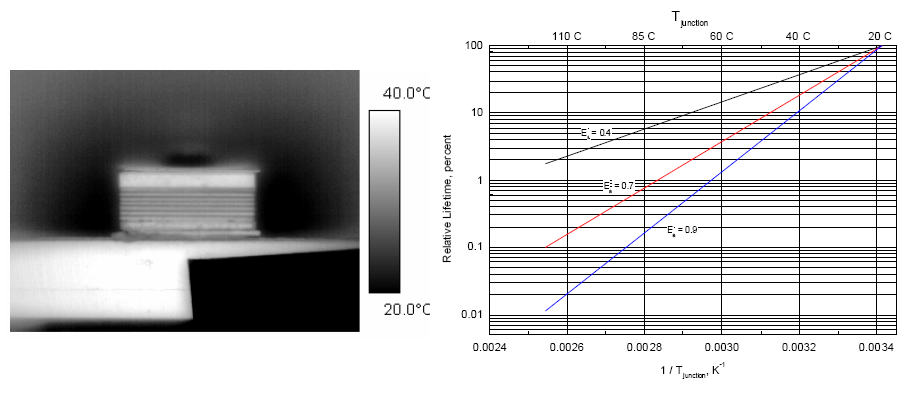
\includegraphics[scale=0.5]{chapters/img/diode_thermal.png} 
\caption{\cite{thermaldiode}}
\label{reliability}
\end{figure}

\textit{\acs{Nd:YAG slab}}. 
The Nd:YAG slab plays a central role in the \acs{laser} configuration. To be able to cope with thermal stresses induced by the wave formation, the slab is thermally bonded to a molybdenum copper block in order to match the thermal expansion coefficients. 

%\begin{figure}[ht!]
%\centering
%\includegraphics[scale=0.5]{chapters/img/Nd-YAG_rthermalconductance.jpg} 
%\caption{}
%\label{reliability}
%\end{figure}

\textit{Electrical Component Temperature Dependency}

\subsection{ Laser Lifetime Expectance} 
\label{opticallifetime}
Multiple aspects influence the expected lifetime of the optical emitter device, such as power, temperature interval, repetition rate and intracavity properties. Since most \acp{laser} have a non-continuous mode of operation (i.e. the duty factor is lower then 100\%), reliability data for long-term cycles are not abundant available.  

For damage-free operation in a harsh, hands-off, environment such as space, a major form of damage risk reduction is the creation of a large intracavity mode to reduce peak fluence. Since resonator efficiency depends strongly on the inversion density of the gain medium, it is advantageous to confine the desired cavity mode as close as possible. To accomplish this, the 808 [nm] light from the diode arrays was collimated by a single plano-convex cylindrical lens made of undoped YAG. By doing this, the probability of the existence of thermal lensing is reduced, increasing the beam quality and the lifetime. 

Considering a constant value of $f_{rep}$ of 5,000 [Hz], the total number of pulses equals $788.4\cdot10^{9}$ [pulses/5 years]. All optical components should be able to cope with the large amount of pulses and the peak power implied by these pulses, i.e. the energy damage threshold of the dielectric components should be higher than the incoming energy of the electromagnetic radiation. Since $I_{p,damage}$) is given with a temporal resolution in the order of a single pulse width ($\sim$10 [ns]), individual pulses can be analyzed. Stationary calculations can be conducted with the information based on the electromagnetic radiation energy and hence, the proper optical elements could be chosen ($I_{p,damage} > I_{p}$).

\cite{nd_yag_life} shows an experimental set-up, where the lifetime of a \acs{DPSSL} is investigated, using approximately the same \acs{laser} configuration with $f_{rep}$ = 242 [Hz] and $E_{p}$ = 0.0150 [J]. The pulse energy is much larger then the value of $E_{p}$ in the case of the \acs{LiDAR} mission described in this report ($\sim$0.001 [J]). \ref{figure} shows the results. After $2.4\cdot10^{9}$ shots, there was no damage found in any of the cavity optics, but inspection of the diodes revealed that a single bas was lost on one array. After the first year, the pump pulse length was increased from 89 [$\mu$m] to 105 [$\mu$m] to restore the output energy to 15 [mJ]. This roughly simulated the procedure that would be performed in space in order to maintain an altimetry link. The final result was that after more than $4.8\cdot10^{9}$ 10 - 15 [mJ] laser pulses, there was no optical damage present in the system \cite{nd_yag_life}. This clearly indicates that the \acp{LDA} lifetime considerations are important for the entire \acs{laser} system. AlGaAs lasers can suffer from catastrophic optical damage (COD), rapid degradation, and gradual degradation. These phenomena are due to darkline defect propagation and a high surface recombination rate \cite{algaas}.

\cite{nd_yag_life} shows an experimental set-up, where the lifetime of a \acs{DPSSL} is investigated, using approximately the same \acs{laser} configuration with $f_{rep} = 242 [Hz]$ and $E_{p} = 0.0150 [J]$. The pulse energy is much larger then the value of $E_{p}$ in the case of the \acs{LiDAR} mission described in this report ($\sim$0.001 [J]). \ref{figure} shows the results. After $2.4\cdot10^{9}$ shots, there was no damage found in any of the cavity optics, but inspection of the diodes revealed that a single bas was lost on one array. After the first year, the pump pulse length was increased from 89 [$\mu$m] to 105 [$\mu$m] to restore the output energy to 15 [mJ]. This roughly simulated the procedure that would be performed in space in order to maintain an altimetry link. The final result was that after more than $4.8\cdot10^{9} 10 - 15 [mJ]$ laser pulses, there was no optical damage present in the system \cite{nd_yag_life}. This clearly indicates that the \acp{LDA} lifetime considerations are important for the entire \acs{laser} system.


\begin{figure}[ht!]
\centering
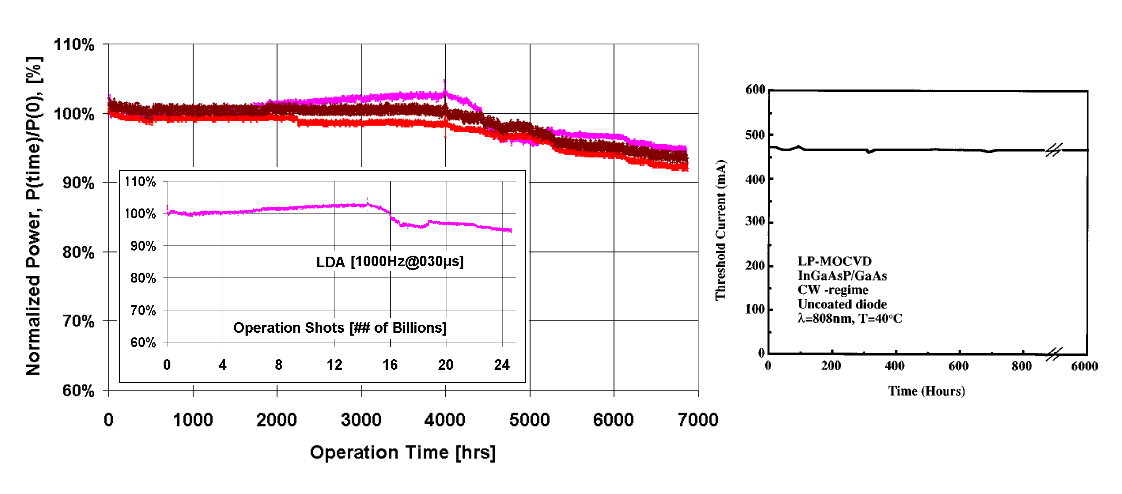
\includegraphics[scale=0.4]{chapters/img/diode_lifetime.png} 
\caption{}
\label{reliability}
\end{figure}

Taken into account the fact that the total number of shots in five years exceed the number of total shots delivered by a single \acs{LDA} without considerable loss in power and beam quality, the obvious consequence is that multiple \acp{LDA} should be implemented within the structure. 

\subsection{\acs{laser} Focus Calculation}
\label{focus}
The figure \ref{fig:EmitterOptics} on page \ref{fig:EmitterOptics} gives a overview of the emitter optics. In order to diverge or focus the laser beam, it is possible to move the parabolic mirror up or down from the exact focus position. In this case, the divergent angle $\gamma$ needs to be calculated, which can be verified or optimized later on to obtain the desired footprint size. The calculation drawing is shown in figure \ref{fig:focus} on page \ref{fig:focus}.

\begin{figure}[ht!]
\centering
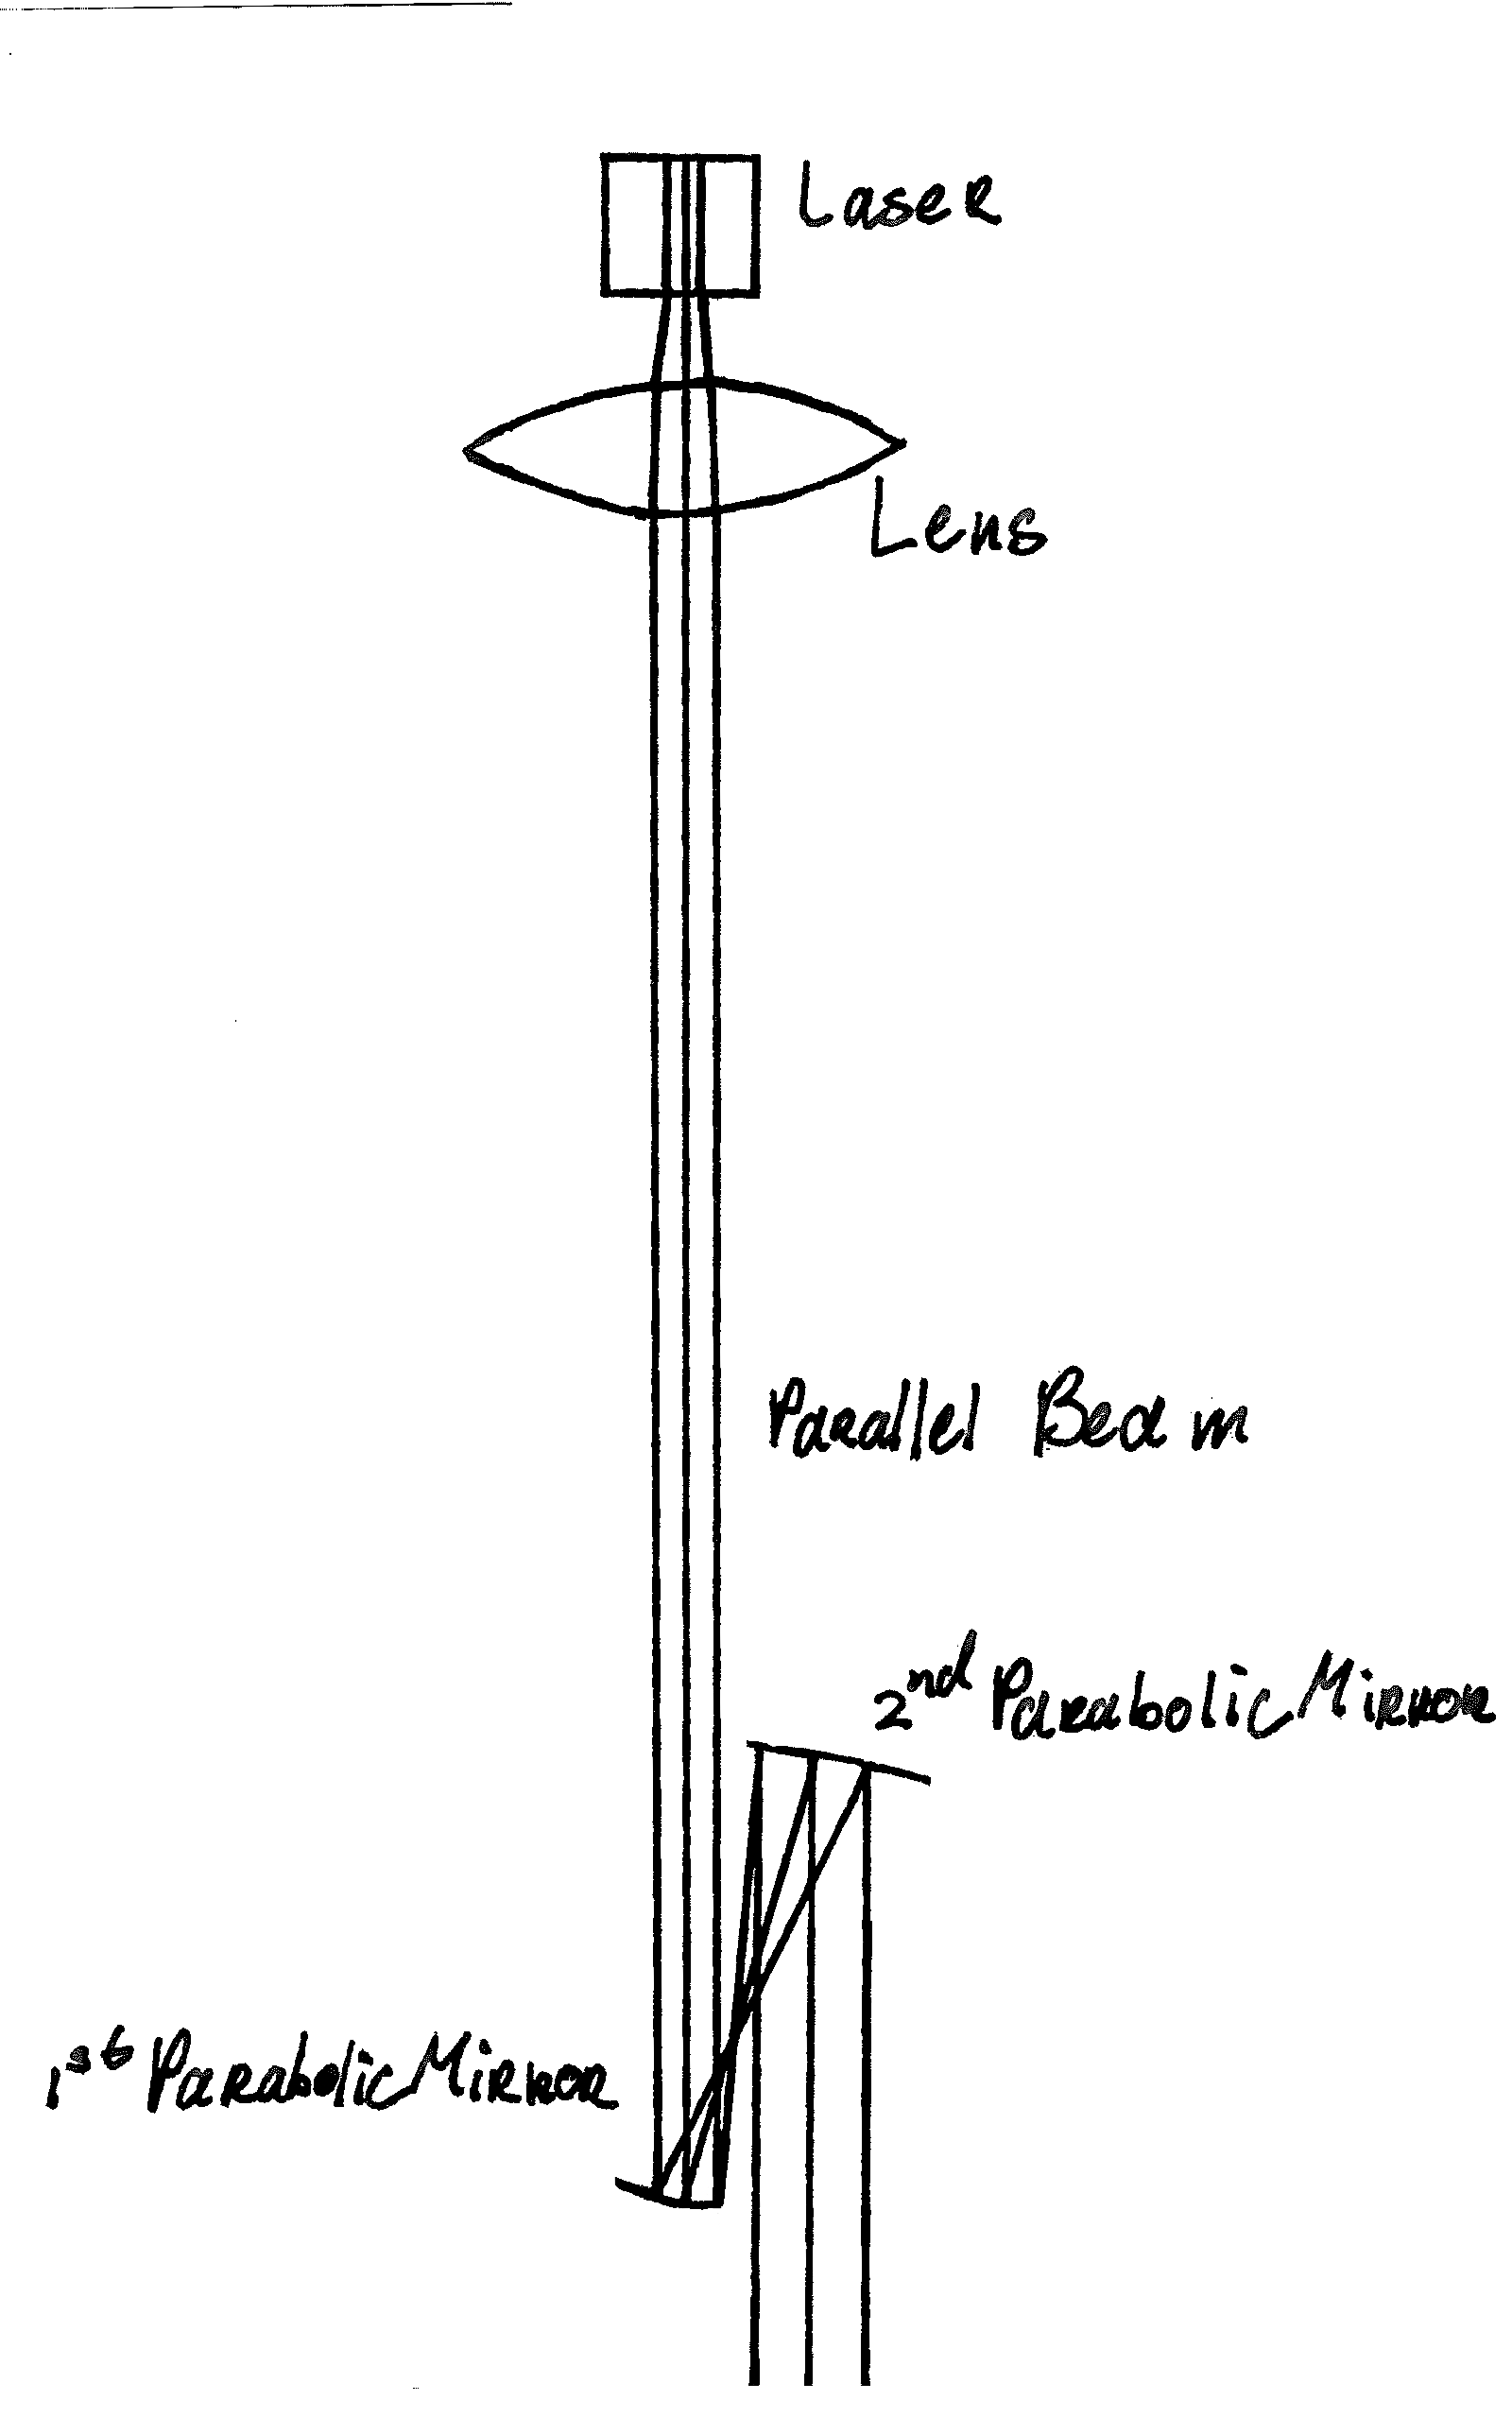
\includegraphics[scale = 0.8]{chapters/img/EmitterOptics.png}
\caption{Emitter optics drawing}
\label{fig:EmitterOptics}
\end{figure}

\begin{figure}[ht!]
\centering
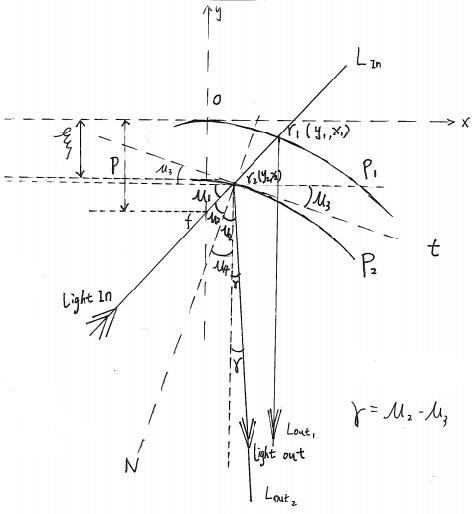
\includegraphics[scale = 1.2]{chapters/img/focus.png}
\caption{Focus calculation draft}
\label{fig:focus}
\end{figure}

In the figure \ref{fig:focus}, $p_{1}$ is the parabolic mirror positioned at the exact focus point f, and p is the distance between f and origin. $p_{2}$ is the parabolic mirror with the exact same shape but which is moved away from focus point with distance $\xi$. $L_{in}$ indicates the incoming light. $L_{out1}$ is the outcoming light due to $p_{1}$ and $L_{out2}$ is the outcoming light due to $p_{2}$. Meanwhile, $r_{1}(x_{1}, y_{1})$, $r_{2}(x_{2}, y_{2})$ are the reflected points due to $p_{1}$ and $p_{2}$. The purpose of this focusing calculation is to find the divergent angle $\gamma$ with respect to the design parameters p, $\xi$ and reflection point $r_{1}(x_{1}, y_{1})$. \cite{parabolic_wiki}Parabolic mirror $p_{1}$ has the equation \ref{p1}, and $p_{2}$ has the equation \ref{p2}. 
\begin{equation}
\label{p1}
y = -\frac{1}{4p}x^{2}
\end {equation}
\begin{equation}
\label{p2}
y = -\frac{1}{4p}x^{2}+\xi
\end {equation}
The equation \ref{Lin} for incoming light line $L_{in}$ can be obtained since $r_{1}(x_{1}, y_{1})$ is known in this case. 
\begin{equation}
\label{Lin}
y = \frac{y_{1}+p}{x_{1}}x-p
\end {equation}
Insert equation \ref{p2} into equation \ref{Lin}, $x_{2}$ of $r_{2}(x_{2}, y_{2})$ can be obtained as:
\begin{equation}
\label{x2}
x_{2} = \frac{-\frac{y_{1}+p}{x_{1}}+\sqrt{{\frac{y_{1}+p}{x_{1}}}^2-\frac{\xi-p}{p}}}{\frac{1}{2p}}
\end {equation}
Next step is to find the tangent line of $p_{2}$ at r2:
\begin{equation}
\label{miu3}
(\frac{dy}{dx})_{x_{2}} = -\frac{1}{2p}x_{2} = tan(\mu_{3}) \Rightarrow \mu_{3} = atan(-\frac{1}{2p}x_{2})
\end {equation}
In the figure, 't' is the tangent line at point $r_{2}$, and 'N' is the normal line perpendicular to the tangent line. The normal line 'N' is also the angle bisect, and $\mu_{2}$ is a half of the reflecting angle. From the drawing, these relations can be found:
\begin{equation}
\label{gamma}
\mu_{1}+\mu_{2}+\mu_{3} = 90^{\circ} = \mu_{1}+\mu_{2}+\mu_{4}
\Longrightarrow \gamma = \mu_{2} - \mu_{4} = \mu_{2} - \mu_{3} 
\end {equation}
To find $\mu_{2}$, $\mu_{1}$ need to be calculated. $\mu_{1}$ is the tangent angle of $L_{in}$ at $r_{1}$ or $r_{2}$:
\begin{equation}
\label{miu2}
(\frac{dy}{dx})_{x_{1},y_{1}} = \frac{y_{1}+p}{x_{1}} = tan(\mu{1})\Rightarrow \mu_{1} = atan(\frac{y_{1}+p}{x_{1}}) \Rightarrow \mu_{2} = 90deg - \mu_{1} - \mu_{3}
\end {equation}
Insert value of $\mu_{2}$ and $\mu_{3}$ to equation \ref{gamma}, so the divergent angle $\gamma = f(p, \xi, r_{1}(x_{1}, y_{1}))$ is obtained. Put these equations into Excel, and it is much easier to see how is $\gamma$ verified. For instance, give values for p=350[mm], $\xi$ = 5[mm] and $x_{1}$=5[mm], $\gamma$=0.01169[deg], which will give the footprint size of 102 meters. By adjusting the $\xi$, the mirror has a divergence of 20.4[m/mm] for the same p and $x_{1}$.

